\documentclass{beamer}

\mode<presentation>
{
  \usetheme{AnnArbor} %Copenhagen
  \usecolortheme{wolverine}
  \setbeamercovered{transparent}
}

\usepackage[english]{babel}
\usepackage[latin1]{inputenc}
\usepackage{times}
\usepackage[T1]{fontenc} 
% Or whatever. Note that the encoding and the font should match. If T1
% does not look nice, try deleting the line with the fontenc.
\usepackage{amsmath}
\usepackage{graphicx}
\usepackage{multirow}

\newcommand{\linespace}{\vskip 0.25cm}

\definecolor{MyForestGreen}{rgb}{0,0.7,0} 
\newcommand{\tableemph}[1]{{#1}}
\newcommand{\tablewin}[1]{\tableemph{#1}}
\newcommand{\tablemid}[1]{\tableemph{#1}}
\newcommand{\tablelose}[1]{\tableemph{#1}}

\definecolor{MyLightGray}{rgb}{0.6,0.6,0.6}
\newcommand{\tabletie}[1]{\color{MyLightGray} {#1}}

% The text in square brackets is the short version of your title and will be used in the
% header/footer depending on your theme.
\title[Morphology in Art Restoration]{Morphological Operations Applied to \\ Digital Art Restoration}

% Sub-titles are optional - uncomment and edit the next line if you want one.
% \subtitle{Why does sub-tree crossover work?} 

% The text in square brackets is the short version of your name(s) and will be used in the
% header/footer depending on your theme.
\author[Dramdahl]{M. Kirbie Dramdahl}

% The text in square brackets is the short version of your institution and will be used in the
% header/footer depending on your theme.
\institute[U of Minn, Morris]
{
  Division of Science and Mathematics \\
  University of Minnesota, Morris \\
  Morris, Minnesota, USA
}

% The text in square brackets is the short version of the date if you need that.
\date[April '14, Sen. Sem., UMM] % (optional)
{29 April 2014 \\ UMM CSci Senior Seminar Conference \\ University of Minnesota, Morris}

% Delete this, if you do not want the table of contents to pop up at
% the beginning of each subsection:
\AtBeginSection[]
{
  \begin{frame}<beamer>
    \frametitle{Outline}
    \tableofcontents[currentsection, hideothersubsections]
  \end{frame}
}

\begin{document}

\begin{frame}
  \titlepage
\end{frame}

% For a 20-25 minute senior seminar talk you probably want something like:
% - Two or three major sections (other than the summary).
% - At *most* three subsections per section.
% - Talk about 30s to 2min per frame. So there should probably be between
%   15 and 30 frames, all told.

\section*{Overview}

\subsection*{Outline}

\begin{frame}
\frametitle{Why?}
Art restoration preserves objects of artistic, cultural, or historical value.
\linebreak
However, this process demands many resources.
\begin{columns}
\begin{column}{0.5\textwidth}
Digital art restoration provides:
\begin{itemize}
\item a comparatively inexpensive alternative,
\item a nondestructive tool, and
\item an approximation of the initial appearance.
\end{itemize}
\end{column}
\begin{column}{0.5\textwidth}
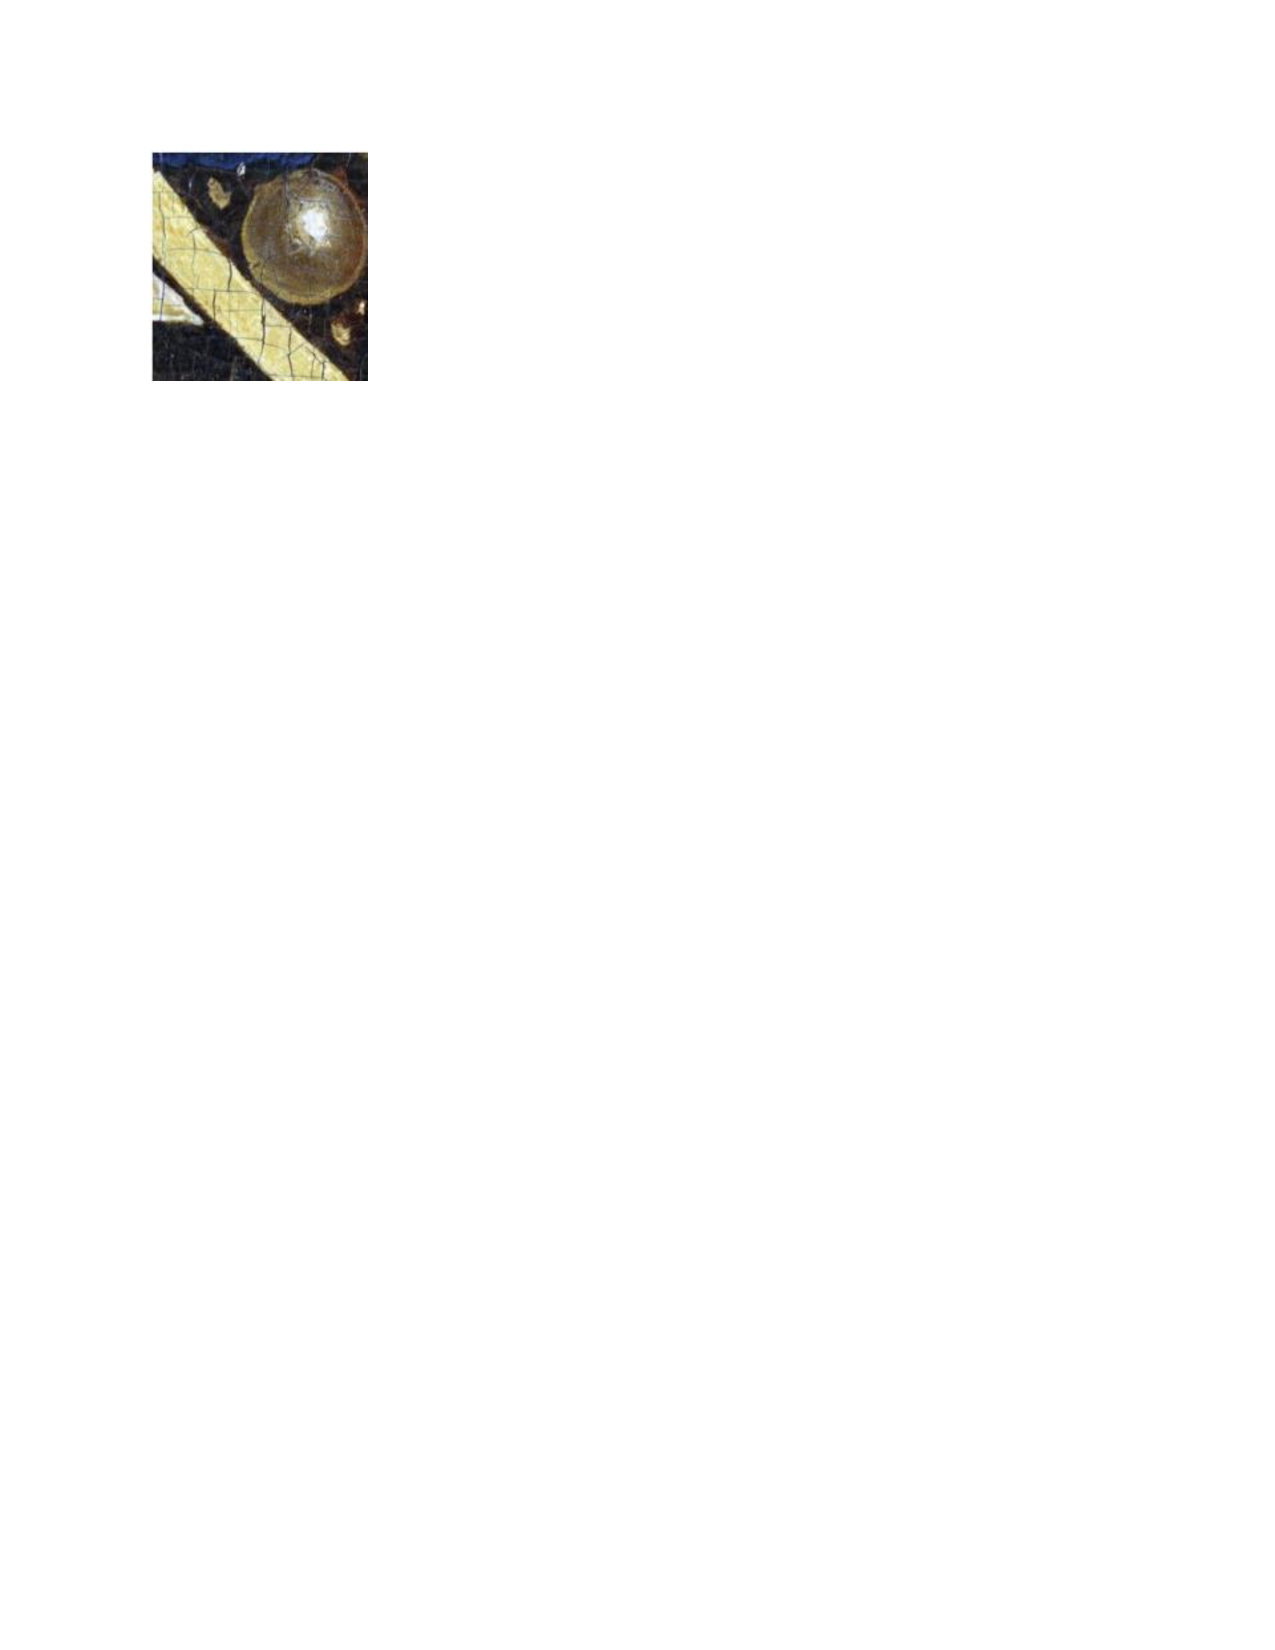
\includegraphics[width=1\textwidth,trim={0.5in 8.4in 5.5in 0.75in},clip]{ghent_altarpiece_original}
\begin{center}
\tiny Cornelis et al
\end{center}
\end{column}
\end{columns}
\end{frame}

\begin{frame}
  \frametitle{Outline}
  \tableofcontents[hideallsubsections]
\end{frame}

\section[Edge Detection]{Edge Detection}

\begin{frame}
\frametitle{Criteria}
Terms
\begin{description}
\item[Edge] boundaries between areas of varying intensity
\item[Intensity] brightness or dullness of a color
\end{description}
\linespace
\linespace
\begin{enumerate}
\item Accuracy \ \ \ \ \ - low error rate
\item Localization \ - minimal distance between detected and actual edge
\item Uniqueness \ - only one response to a single edge
\end{enumerate}
\end{frame}

\begin{frame}
\frametitle{Canny Algorithm}
{\Large Note: Break into multiple slides and add images.}
\linebreak
\begin{enumerate}
\item Smooth image.
\linebreak
\item Find jumps in intensity.
\linebreak
\item Search regions for local maximum.
\linebreak
\item Compare intensity of remaining pixels to two thresholds.
\end{enumerate}
\end{frame}

\section[Morphological Operations]{Morphological Operations}

\begin{frame}
\frametitle{Morphological Operations}
\begin{columns}
\begin{column}{0.5\textwidth}
Binary and Greyscale Images
\linebreak
\linebreak
Two Inputs:
\begin{itemize}
\item original image
\item structuring element
\end{itemize}
\end{column}
\begin{column}{0.5\textwidth}
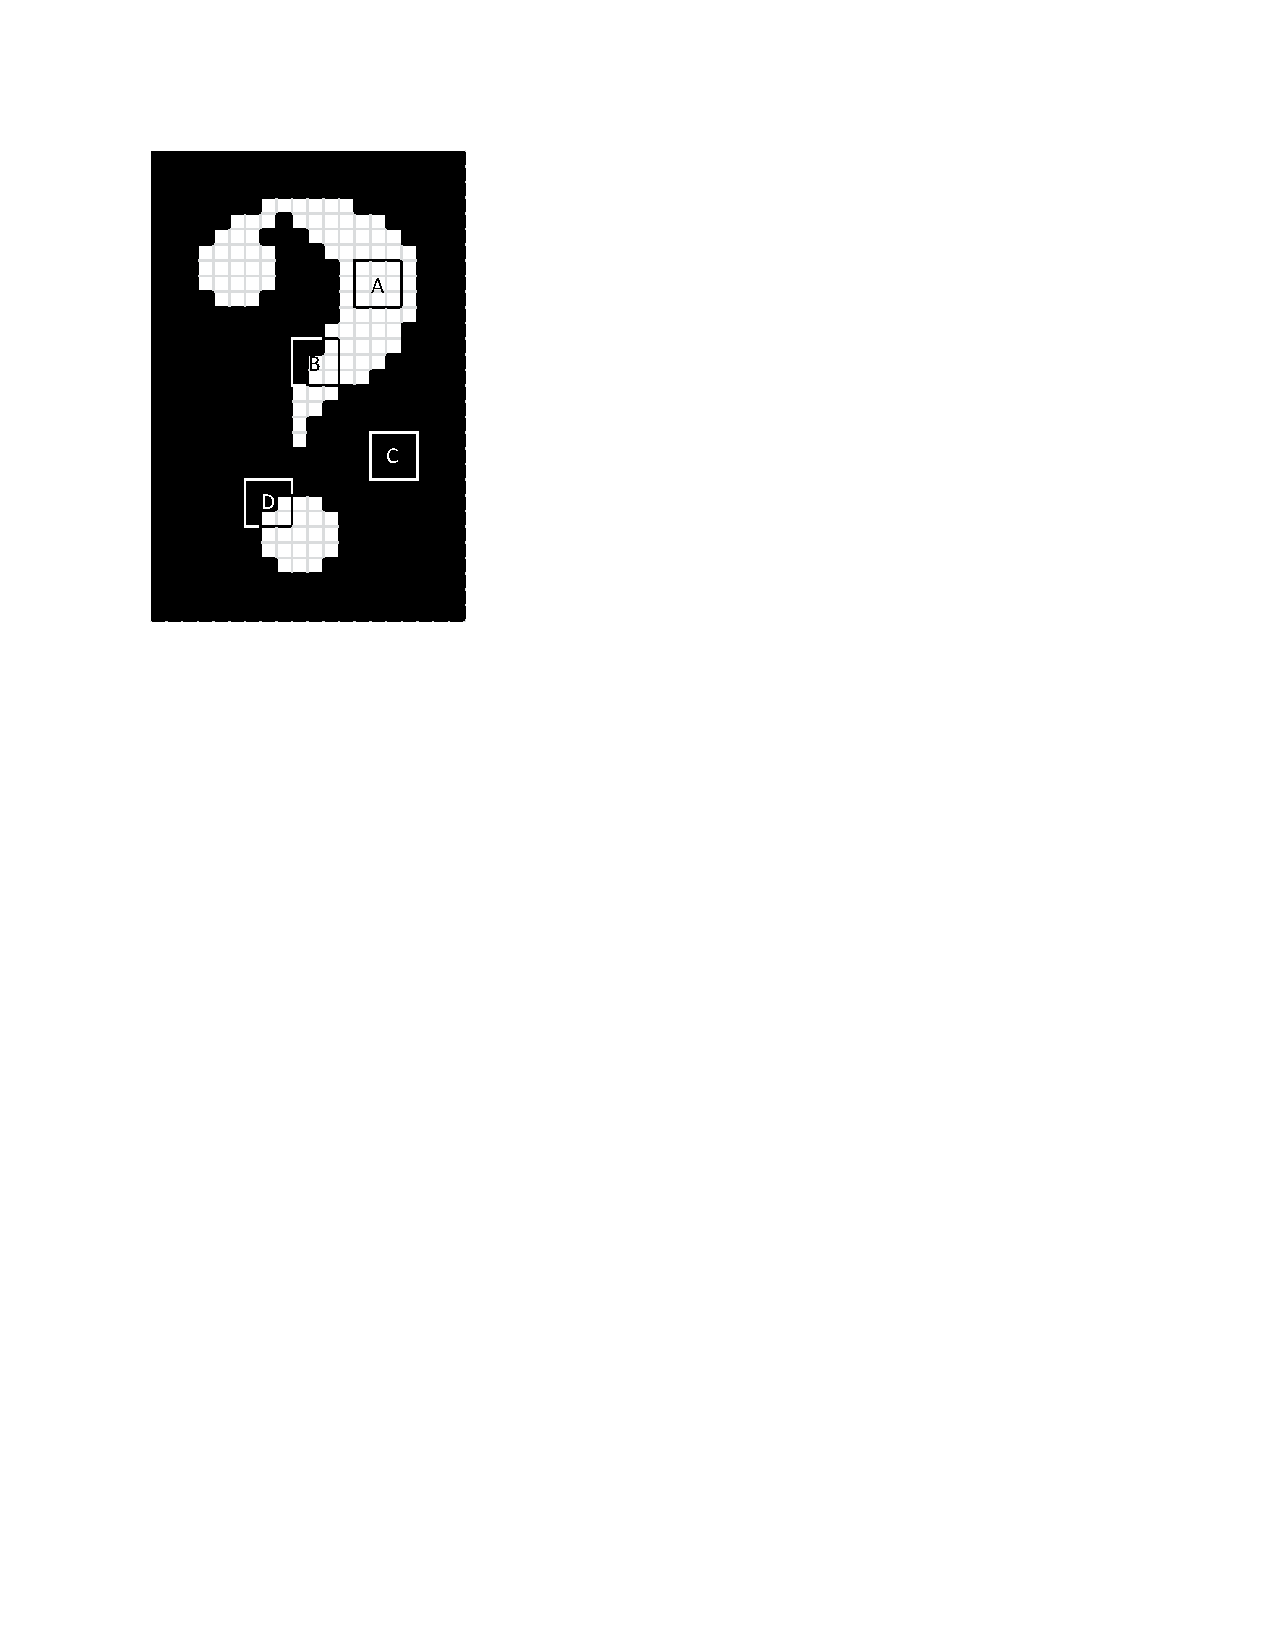
\includegraphics[width=1\textwidth,trim={0 6.5in 4in 0},clip]{structuring_element_placement}
\end{column}
\end{columns}
\end{frame}

\subsection[Erosion]{Erosion}

\begin{frame}
\frametitle{Erosion}
{\Large Note: Make transparency for structuring element.}
\begin{center}
Erosion removes foreground pixels.
\begin{equation*}
g = f \ominus s
\end{equation*}
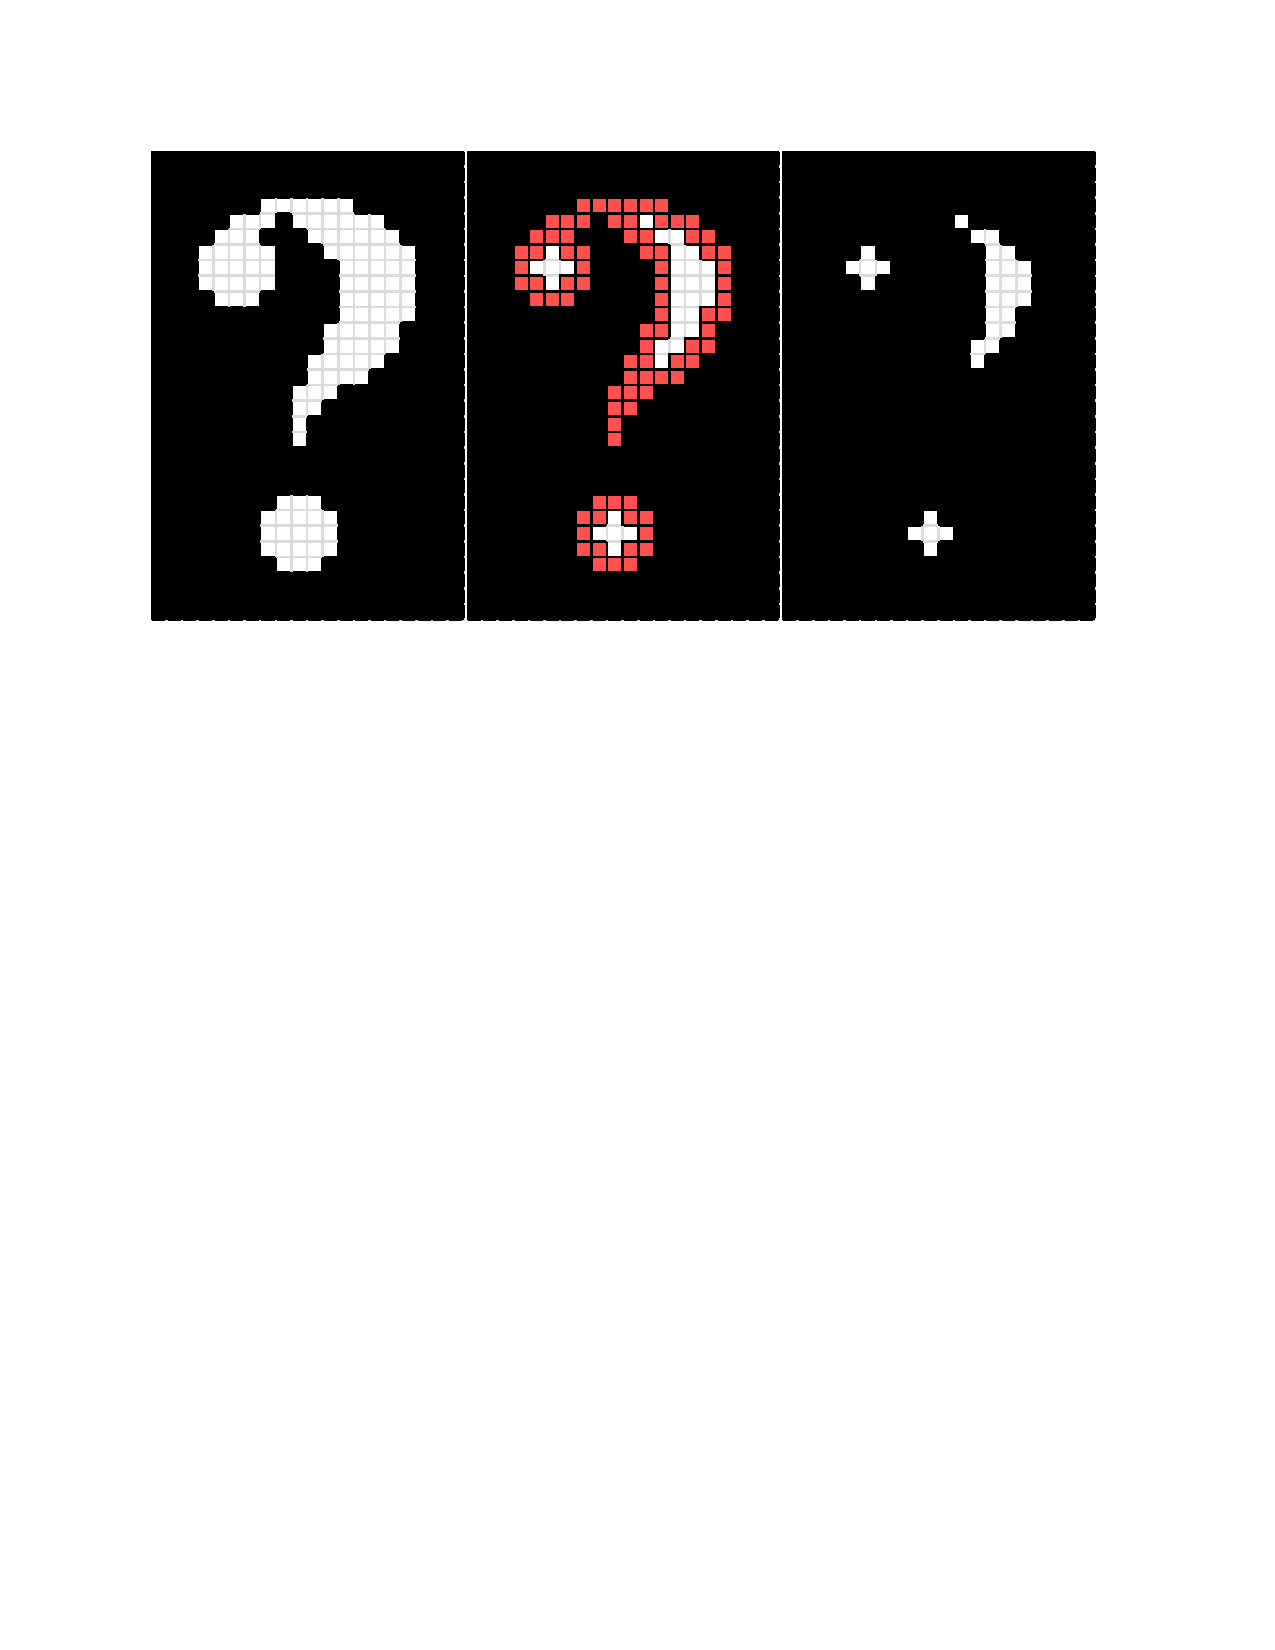
\includegraphics[width=1\textwidth,trim={0 0 0 0.5in},clip]{erosion}
\end{center}
\end{frame}

\subsection[Dilation]{Dilation}

\begin{frame}
\frametitle{Dilation}
\begin{center}
Dilation adds foreground pixels.
\begin{equation*}
g = f \oplus s
\end{equation*}
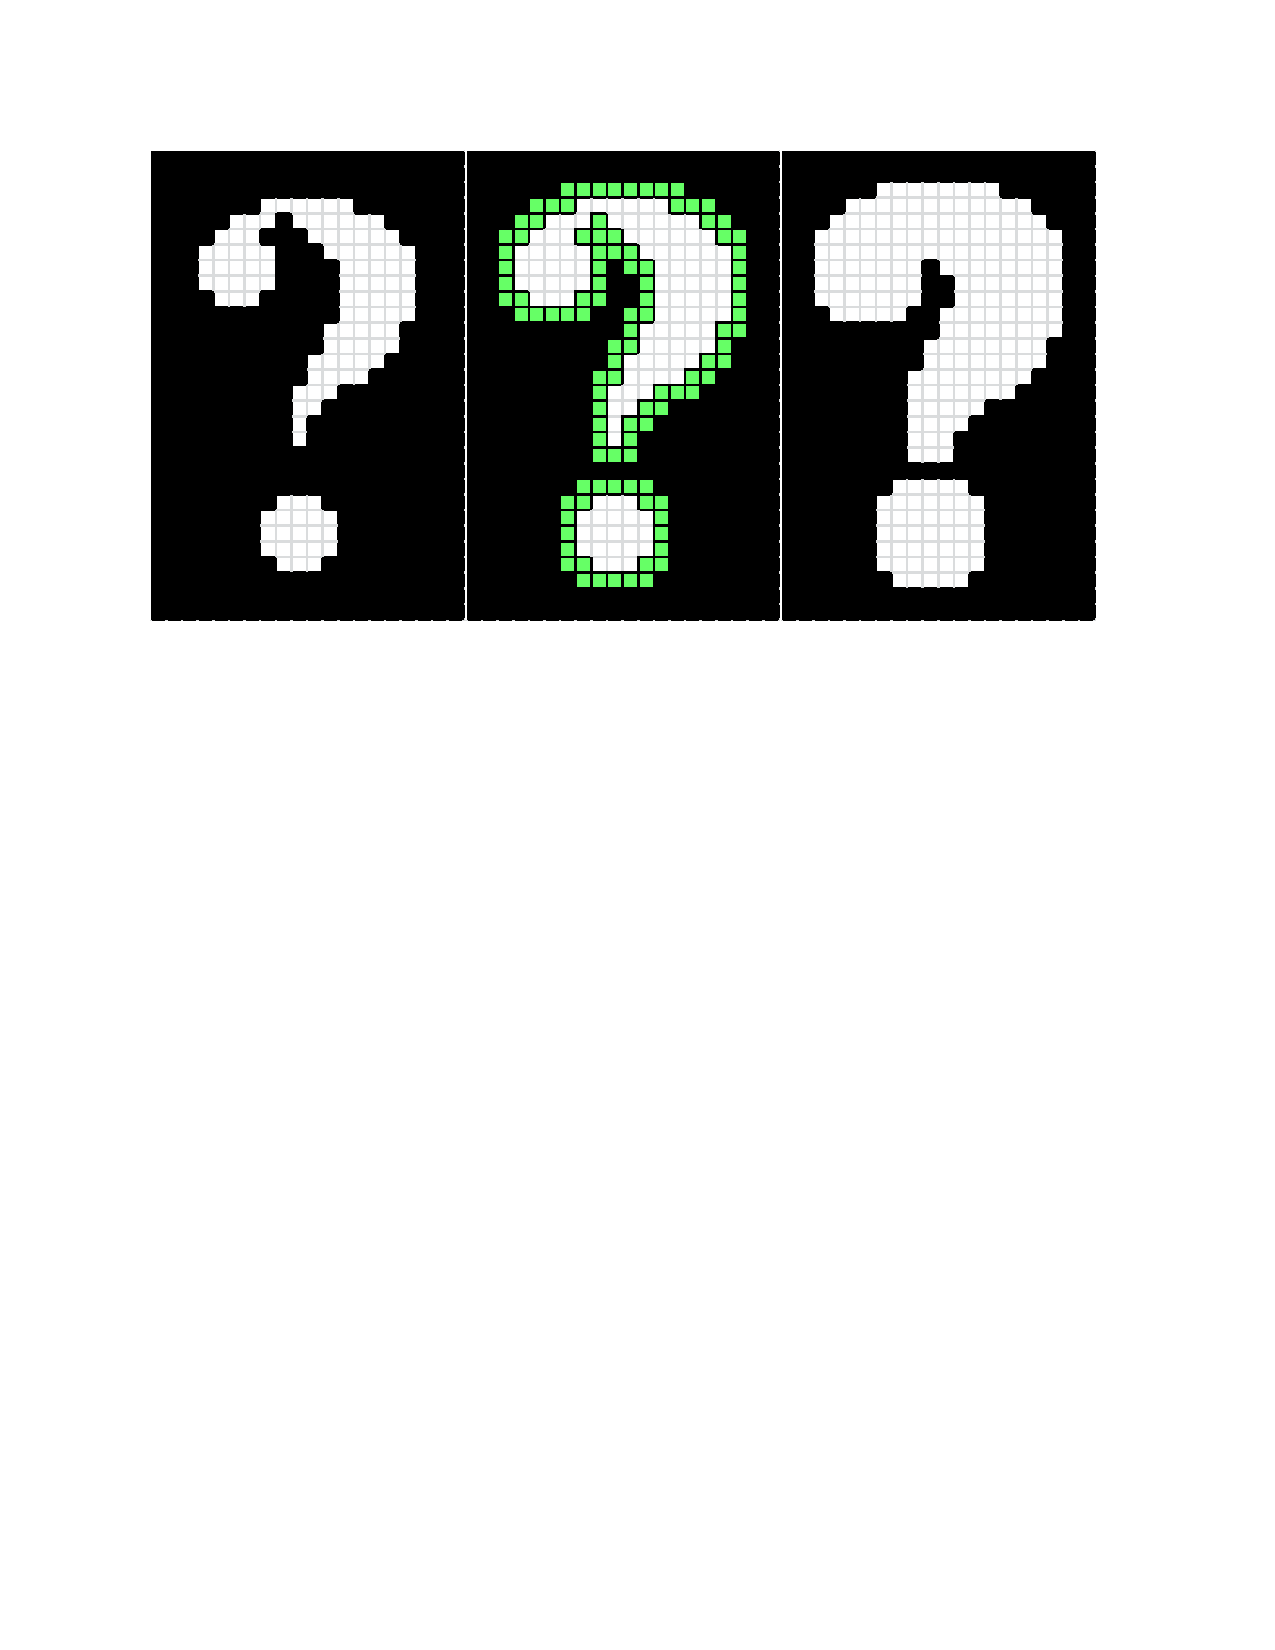
\includegraphics[width=1\textwidth,trim={0 0 0 0.5in},clip]{dilation}
\end{center}
\end{frame}

\subsection[Opening]{Opening}

\begin{frame}
\frametitle{Opening}
{\Large Note: Make transparency for structuring element.}
\begin{center}
Opening removes foreground pixels... neatly.
\begin{equation*}
g = f \circ s = (f \ominus s) \oplus s
\end{equation*}
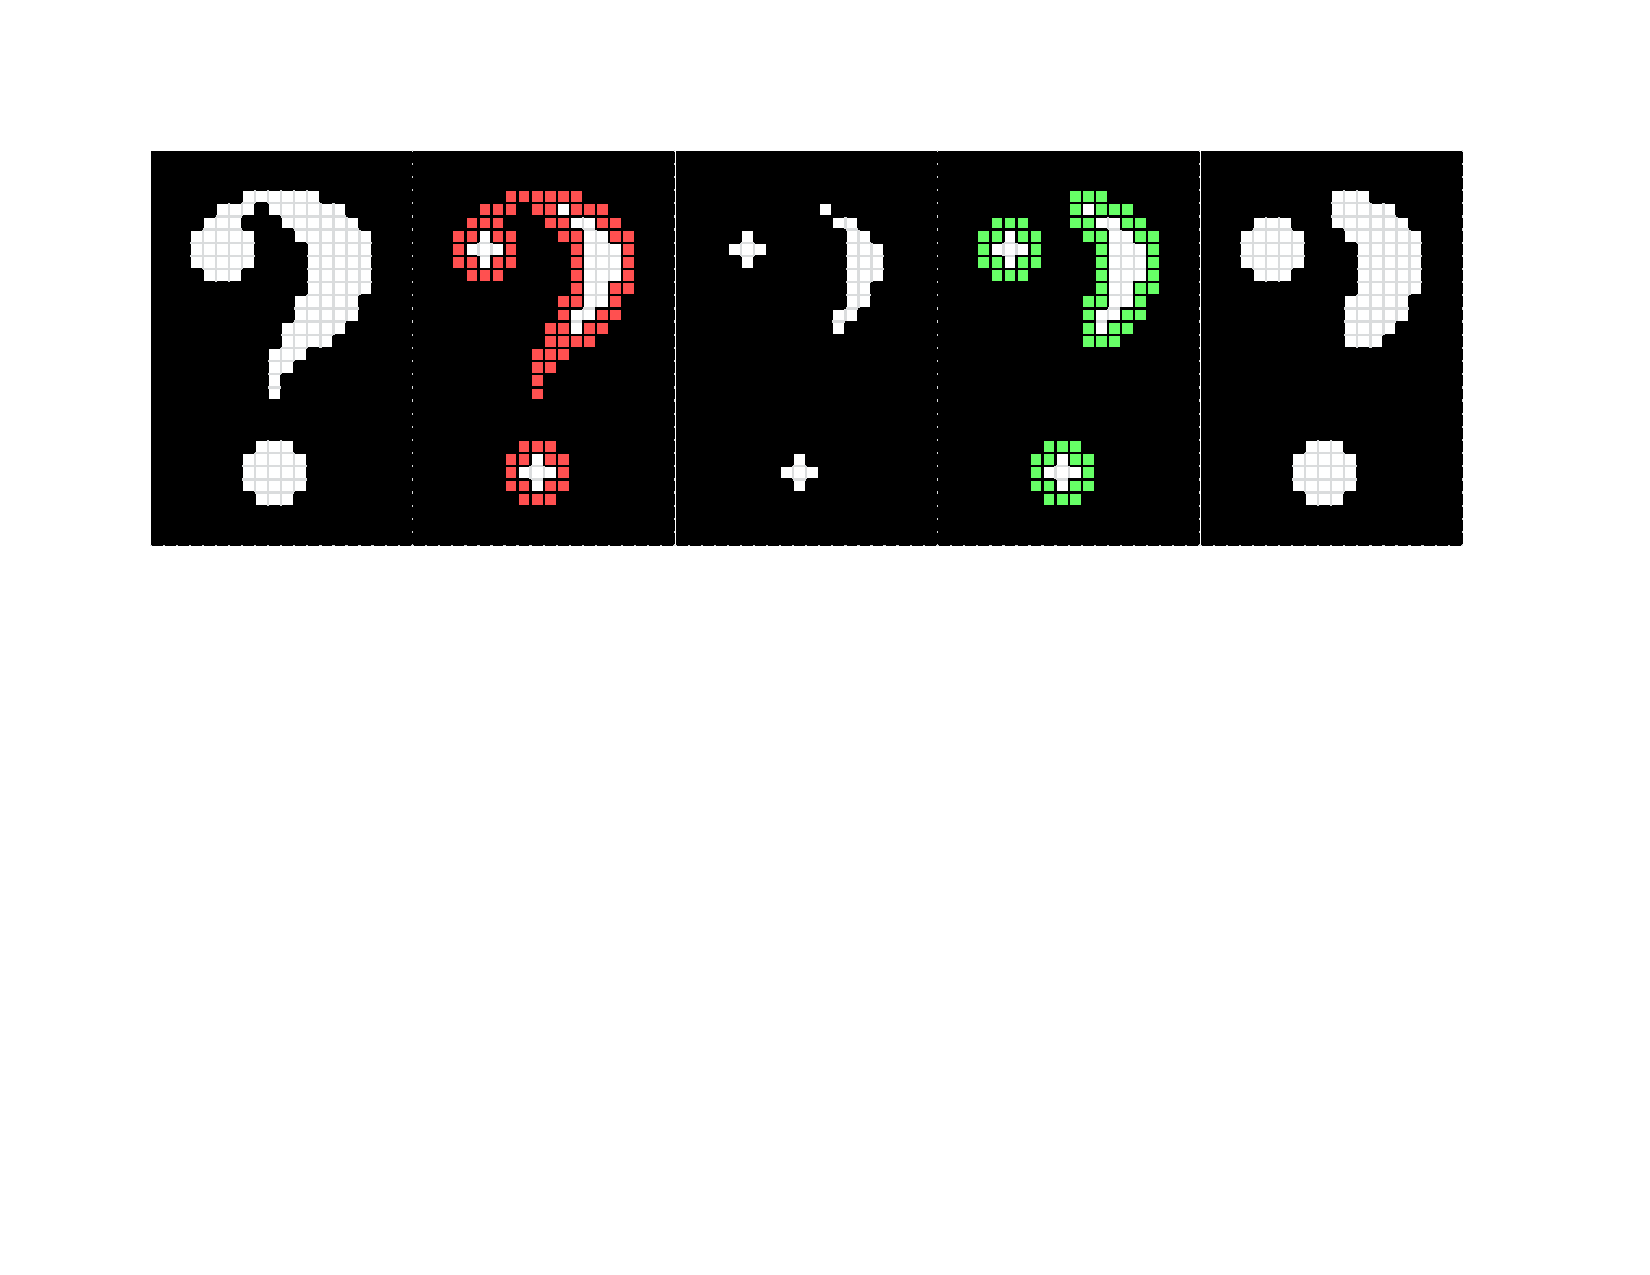
\includegraphics[width=1\textwidth,trim={0 0 0 0.5in},clip]{opening}
\end{center}
\end{frame}

\subsection[Closing]{Closing}

\begin{frame}
\frametitle{Closing}
\begin{center}
Closing adds foreground pixels... neatly.
\begin{equation*}
g = f \bullet s = (f \oplus s) \ominus s
\end{equation*}
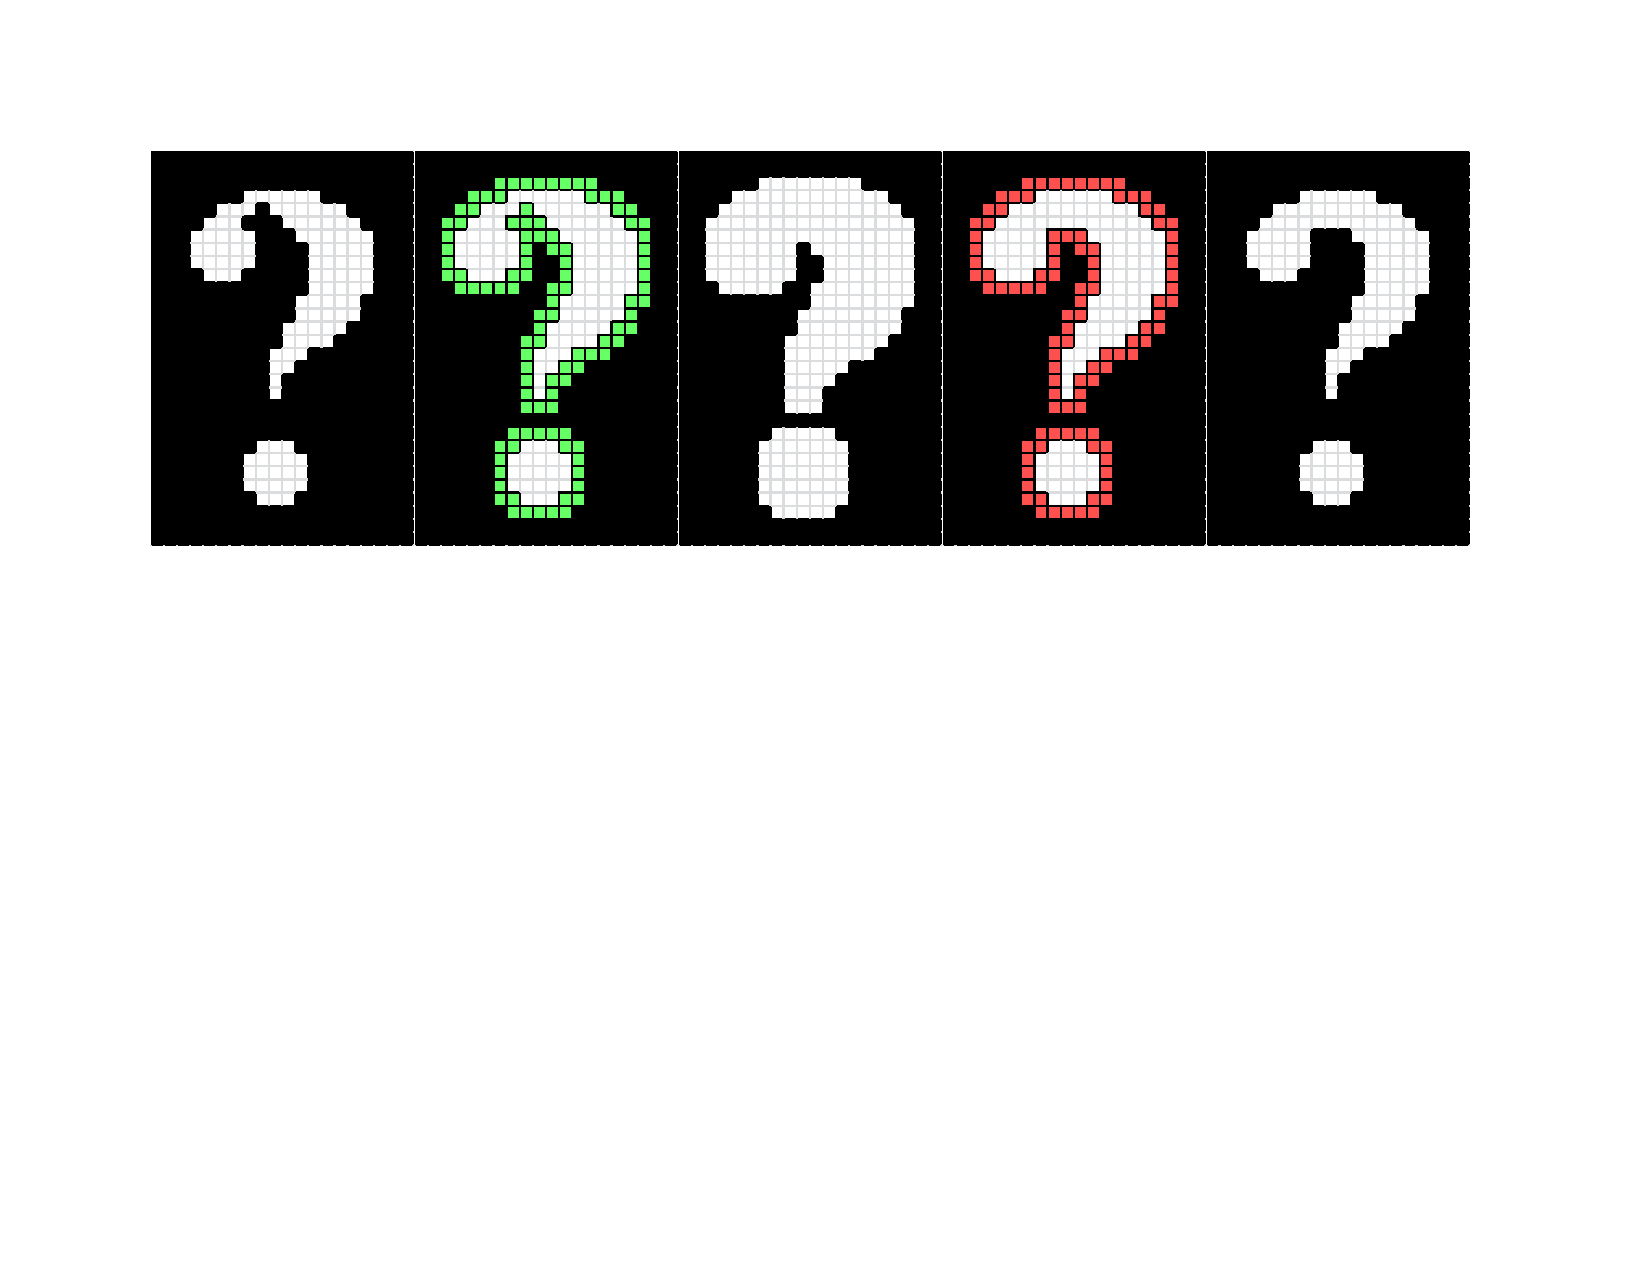
\includegraphics[width=1\textwidth,trim={0 0 0 0.5in},clip]{closing}
\end{center}
\end{frame}

\section[Methods of Crack Detection]{Methods of Crack Detection}

\subsection[Top-Hat Transform]{Top-Hat Transform}

\begin{frame}
\frametitle{Top-Hat Algorithm}
\begin{columns}
\begin{column}{0.5\textwidth}
\begin{description}
\item[Black Top-Hat] \hfill \\ darker details on lighter background
\end{description}
\begin{equation*}
BTH = (f \bullet s) - f
\end{equation*}
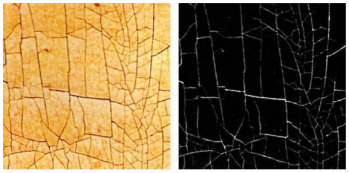
\includegraphics[width=1\textwidth]{black_top_hat}
\begin{center}
\tiny Spagnolo and Somma
\end{center}
\end{column}
\begin{column}{0.5\textwidth}
\begin{description}
\item[White Top-Hat] \hfill \\ lighter details on darker background
\end{description}
\begin{equation*}
WTH = f - (f \circ s)
\end{equation*}
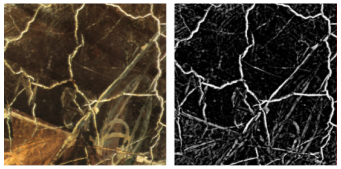
\includegraphics[width=1\textwidth]{white_top_hat}
\begin{center}
\tiny Spagnolo and Somma
\end{center}
\end{column}
\end{columns}
\end{frame}

\subsection[Alternative Method]{Alternative Method}

\begin{frame}
\frametitle{Alternative Method}
{\Large Note: Break into multiple slides, add images, and possibly a diagram.}
\begin{enumerate}
\item Set threshold; pixels exceeding threshold are determined to be cracks.
\item Closing is applied to image, grouping isolated pixels.
\item Previous two steps form binary crack mask.
\item Canny edge detection algorithm implemented on original image to obtain edge mask.
\item Dilation applied to edge mask.
\item Crack and edge mask joined to form binary mask.
\item Binary mask iteratively eroded until certain percentage of edge information is lost.
\end{enumerate}
\end{frame}

\section[Inpainting]{Inpainting}

\begin{frame}
\frametitle{Inpainting Process}
{\Large Note: Break into multiple slides and add images.}
The image is broken down into regions, which are further broken down into neighborhoods. For each defective pixel $i$:
\begin{enumerate}
\item Find the context of $i$.
\item Examine all other neighborhoods within the region of $i$.
\item Find neighborhood most similar to context of $i$ by sum of squared differences.
\item If the sum of squared errors is below a set threshold, replace all defective pixels in the neighborhood of $i$ with corresponding pixels from most similar neighborhood.
\item Otherwise, replace pixel $i$ with the median value of all non-defective pixels within its neighborhood.
\end{enumerate}
\end{frame}

\section[Results]{Results}

\begin{frame}
\frametitle[Definitions]{Definitions}
\begin{columns}
\begin{column}{0.5\textwidth}
Categories:
\begin{itemize}
\item true positives (\textit{tp})
\item false positives (\textit{fp})
\item true negatives (\textit{tn})
\item false negatives (\textit{fn})
\end{itemize}
\end{column}
\begin{column}{0.5\textwidth}
Equations:
\begin{itemize}
\item False and True Positive Rate
\begin{equation*}
FP = fp / (fp + tn)
\end{equation*}
\begin{equation*}
TP = tp / (tp + fn)
\end{equation*}
\item Precision and Recall
\begin{equation*}
P = tp / (tp + fp)
\end{equation*}
\begin{equation*}
R = tp / (tp + fn)
\end{equation*}
\end{itemize}
\end{column}
\end{columns}
\end{frame}

\begin{frame}
\frametitle[Statistics]{Statistics}
\begin{table}
\centering
\resizebox{10cm}{!}{
\begin{tabular}{|l|l|r|r|r|r|r|r|r|}
\hline
\textbf{Method} & \textbf{Classification} & \textbf{\textit{tp}} & \textbf{\textit{fn}} & \textbf{\textit{tn}} & \textbf{\textit{fp}} & \textbf{\textit{TP} (or \textit{R})} & \textbf{\textit{FP}} & \textbf{\textit{P}}\\ \hline
\multirow{8}{*}{Top-Hat Transform}
& Crack Thickness - Thin & 220 & 30 & 230 & 20 & 0.880 & 0.080 & 0.917\\ \cline{2-9}
& Crack Thickness - Medium & 232 & 18 & 231 & 19 & 0.928 & 0.076 & 0.924\\ \cline{2-9}
& Crack Thickness - Thick & 235 & 15 & 238 & 12 & 0.940 & 0.048 & 0.951\\ \cline{2-9}
& Number of Cracks - Few & 242 & 8 & 245 & 5 & 0.968 & \textbf{0.020} & 0.980\\ \cline{2-9}
& Number of Cracks - Medium & 245 & 5 & 241 & 9 & \textbf{0.980} & 0.036 & 0.965\\ \cline{2-9}
& Number of Cracks - Many & 243 & 7 & 243 & 7 & 0.972 & 0.028 & 0.972\\ \cline{2-9}
& Crack Connectivity - Low & 215 & 35 & 219 & 31 & \textbf{0.860} & \textbf{0.124} & 0.874\\ \cline{2-9}
& Crack Connectivity - High & 218 & 32 & 221 & 29 & 0.872 & 0.116 & 0.883\\ \hline
\multirow{3}{*}{Alternative Method}
& Edge Information Lost - 1\% & - & - & - & - & \textbf{0.932} & - & \textbf{0.497}\\ \cline{2-9}
& Edge Information Lost - 30\% & - & - & - & - & 0.857 & - & 0.594\\ \cline{2-9}
& Edge Information Lost - 70\% & - & - & - & - & \textbf{0.530} & - & \textbf{0.704}\\ \hline
\end{tabular}
}
\end{table}
\begin{center}
\huge ADD GRAPH HERE!!!
\end{center}
\end{frame}

\begin{frame}
\frametitle[Results]{Results}
\begin{columns}
\begin{column}{0.5\textwidth}
Original Image
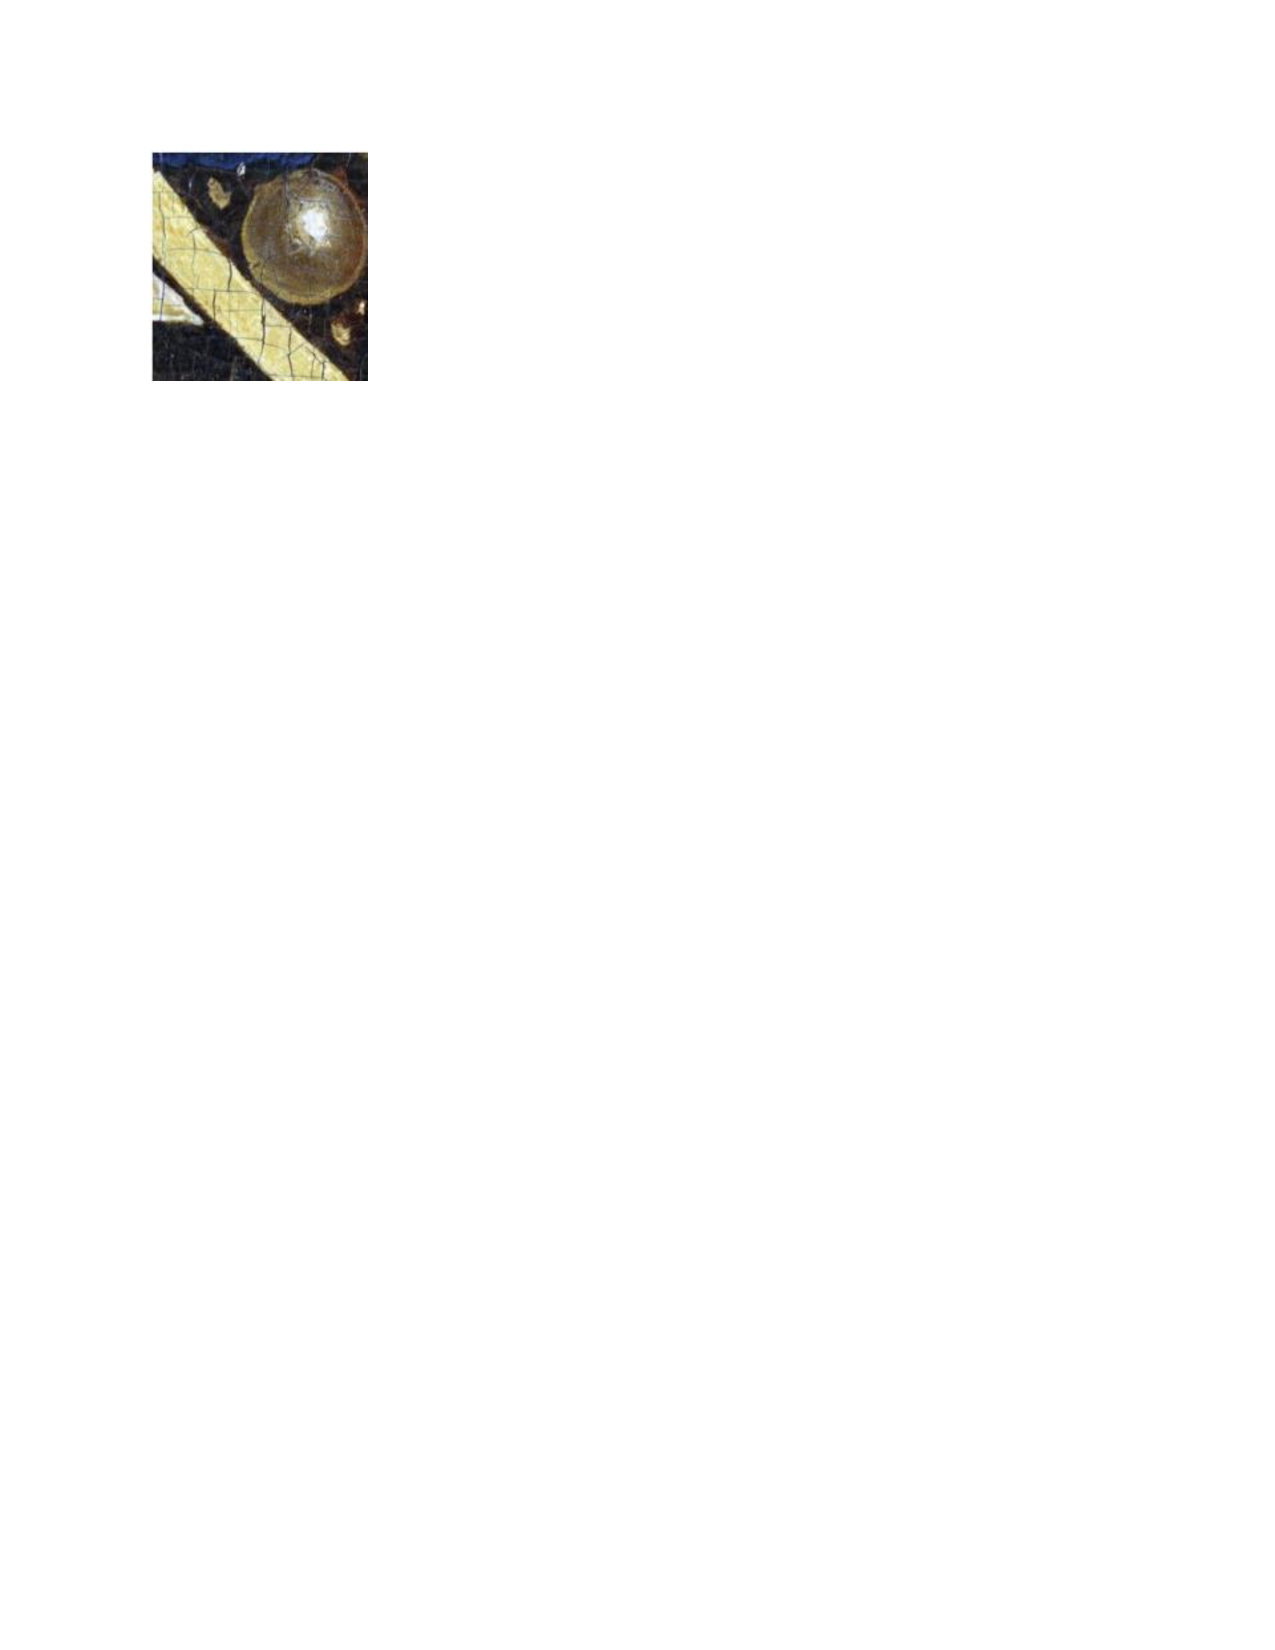
\includegraphics[width=1\textwidth,trim={0.5in 8.4in 5.5in 0.75in},clip]{ghent_altarpiece_original}
\begin{center}
\tiny Cornelis et al
\end{center}
\end{column}
\begin{column}{0.5\textwidth}
Restored Image
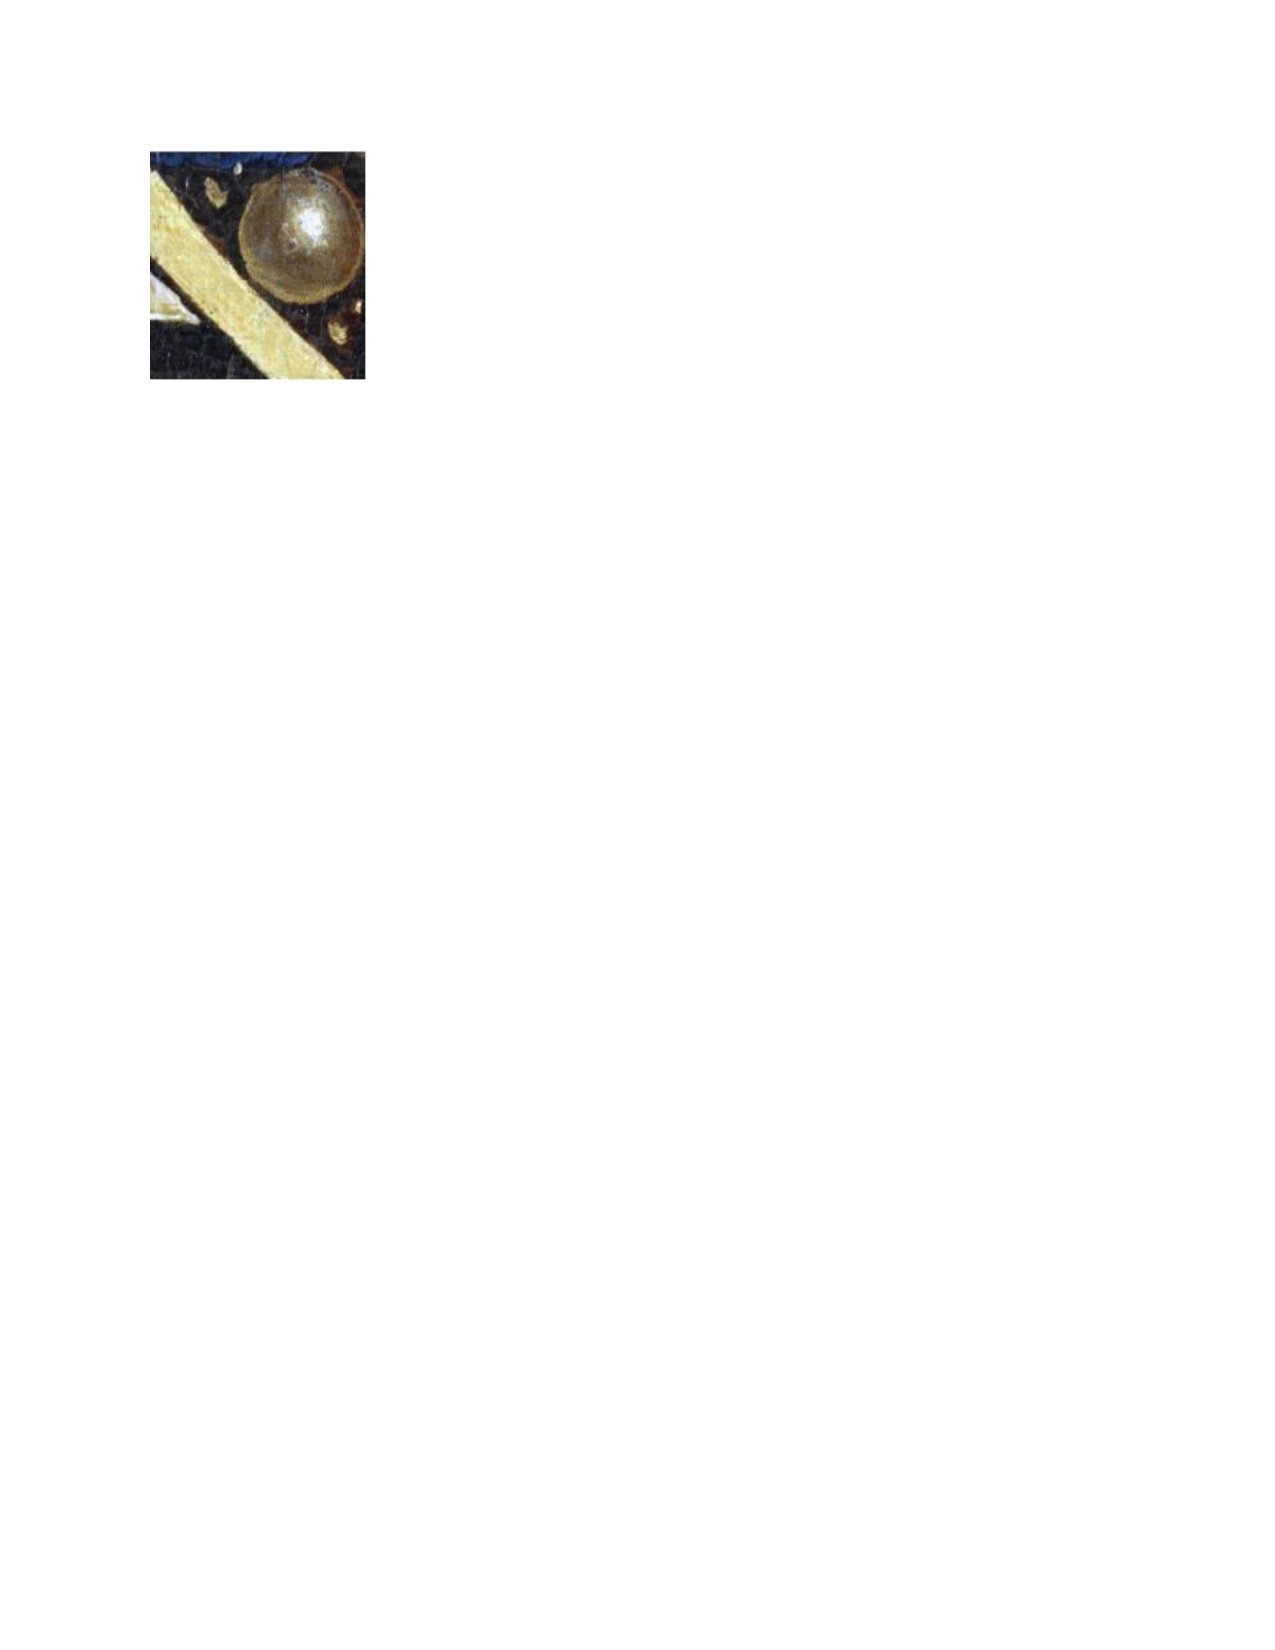
\includegraphics[width=1\textwidth,trim={0.5in 8.4in 5.5in 0.75in},clip]{ghent_altarpiece_restored}
\begin{center}
\tiny Cornelis et al
\end{center}
\end{column}
\end{columns}
\end{frame}

\section[Conclusions]{Conclusions}

\begin{frame}
\frametitle[Conclusions]{Conclusions}
The top-hat transform has been demonstrated to outperform the alternative examined here.
\linebreak
\linebreak
\linebreak
Further Work:
\begin{itemize}
\item Implement other methods of crack detection.
\item Examine effects of various forms of edge detection and inpainting.
\item Study the detection and removal of other defects.
\end{itemize}
\end{frame}

\begin{frame}
\frametitle{Thanks!}
\linespace
\linespace
%Contact: \texttt{dramd002@morris.umn.edu}
\linespace
\linespace
\begin{center}
{\huge Questions?}
\end{center}
\end{frame}

\section*{References}

\begin{frame}[allowframebreaks] 
\frametitle{References} 
\nocite{*}
\bibliographystyle{abbrv}
{\tiny \bibliography{paper}}
\end{frame}

\end{document}